\documentclass{beamer}
  \usepackage[english]{babel}
  \usepackage[utf8]{inputenc}
  \usepackage{times}
  \usepackage{amsmath,amsthm, amssymb, latexsym,ragged2e}
  \boldmath
  \usepackage{multicol}
  
  \usetheme{Poster}
  \usepackage[orientation=portrait,size=a0,scale=1.4]{beamerposter}


% Urban systems have their own complexity and specific characteristics, but still have been described and modelled using analogies and models imported from other disciplines. In particular, biological metaphors have been widely used in urban planning and design. We argue that fruitful transfer of concepts between biology and urban science can be achieved within a complexity interdisciplinary framework. We illustrate this idea by synthesising a recent stream of research focusing on urban morphogenesis, urban evolution and urban co- evolution. First, urban morphogenesis can be understood as the growth of urban form, at the scale of a city or an urban area. [1] compares and calibrates morphogenesis models at the district scale. [2] shows for urban areas in Europe that reaction-diffusion models can accurately reproduce existing urban forms. Then, the concept of urban evolution can be related to cultural evolution in urban systems, but also to cities themselves as evolving entities. [3] proposed an evolutionary theory of cities to understand the dynamics of urban systems, in the sense of adaptive complex systems. In that context, a model of urban evolution is introduced by [4] in which the main ingredients are innovations propagating between cities. Finally, [5] introduces a multi-level definition for a concept of urban co- evolution, with at the intermediate level the possibility of statistically co-evolving population of urban entities within territorial niches. A method to characterise it on spatio-temporal data was introduced by [6]. At the mesoscopic scale of urban areas, the morphogenesis model of [7] effectively captures such a co-evolution between indicators of urban morphology and the topology of road networks. At the macroscopic scale of the system of cities, [8] study a co- evolution model between cities and inter-city networks, and show that diverse regimes of co- evolution can be produced. We suggest that other several interdisciplinary bridges could be relevant to urban science. For example, biomimicry has been put forward as an effective tool for urban design and architecture, while the concept of autopoiesis has not been applied yet to urban systems. Urban computing and collective intelligence, as research fields such as smart cities and digital twins are emerging, may also be linked to studies of collective computation in biological systems. Altogether, understanding urban systems as complex systems implies an interdisciplinary integration of concepts, methods and models.


  \title{Morphogenesis, Evolution and Co-evolution of Cities}
  \author[juste.raimbault@polytechnique.edu]{J. Raimbault$^{1,2,3}$}
  \institute[]
  {$^1$ CASA, UCL; $^2$ UPS CNRS 3611 ISC-PIF; $^3$ UMR CNRS 8504 Géographie-cités\vspace{1cm}}
  \date{}
  
  \logo{
  \hfill
  
\includegraphics[height=8cm]{figures/ucl-logo-colours-notext.jpg}
  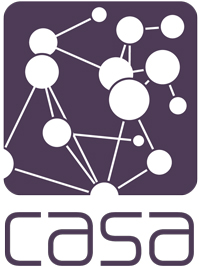
\includegraphics[height=8cm]{figures/casa_logo.jpeg}
  %
\includegraphics[height=8cm]{figures/isc}
  %
\includegraphics[height=8cm]{figures/geocite}
  \hfill\hfill
  }


  %%%%%%%%%%%%%%%%%%%%%%%%%%%%%%%%%%%%%%%%%%%%%%%%%%%%%%%%%%%%%%%%%%%%%%%%%%%%%%%%%5
  \begin{document}
  \begin{frame}{} 
  
    \vfill
    \begin{columns}[t]
      \begin{column}{.49\textwidth}
      
      \vspace{-1cm}
      
        \begin{block}{Context}
        \vspace{-1cm}
        \begin{columns}[t]
        \begin{column}{.95\textwidth}
          \begin{itemize}         
          \item \justify Urban complexity and interdisciplinarity \cite{pumain2005cumulativite}
          \end{itemize}
          \bigskip
          \begin{itemize} 
          \item \begin{justify} Urban science and Artificial Life: applications of biological concepts in planning and design \cite{batty2009centenary}
          \end{justify}
          
          \end{itemize}
          
          \bigskip
          \begin{justify}
          $\rightarrow$ \textit{Urban morphogenesis, urban evolution and urban co-evolution as concepts to understand urban dynamics and sustainability}
          \end{justify}
          
          \end{column}
          \end{columns}
        \end{block}
        
         \begin{block}{Urban morphogenesis}
         % Urban morphogenesis can be in it simplest sense understood as the growth of urban form, at the scale of a city or an urban area. Raimbault et al. (2014) introduce for example a cellular automaton coupled with a dynamical road net- work, which produces a variety of dynamical regimes of ur- ban growth (Raimbault, 2017). Raimbault and Perret (2019) compare and calibrate generative models at the district scale. Raimbault (2018d) show the complementarity of multiple heuristics to simulate the morphogenesis of transportation networks. The concept of urban morphogenesis can also be made closer to its biological counterpart by showing how reaction-diffusion models can accurately reproduce existing urban forms, as shown by Raimbault (2018a) for urban areas in Europe. Finally, by constructing a definition of urban morphogenesis as the strong coupling between the growth of urban form and the emergence of urban functions, Raim- bault (2018b) introduces an original viewpoint in which the transfer from biology is crucial. Following this positioning, the morphogenesis model studied by Raimbault (2019) uses transportation network to integrate a functional aspect into the dynamics of urban growth. Processes of urban morpho- genesis can be seen as occurring within territorial niches (Holland, 2012), what suggests the relevance of studying urban evolution within and between these niches at larger scales.

        %\vspace{-1cm}
        \begin{columns}[t]
        \begin{column}{.95\textwidth}
        \vspace{-2cm}
        
        %\begin{justify}
          \textbf{Definition of urban morphogenesis} \cite{raimbault2018caracterisation}: \textit{strong coupling between the dynamics of urban form and function}
          
          \bigskip
          
          \textbf{Generative models} for urban morphogenesis:
          
          \begin{itemize}
          		\item cellular automaton and road network \cite{raimbault2014hybrid}
          		\item building configurations \cite{raimbault2019generating}
          		\item reaction-diffusion model for population density \cite{raimbault2018calibration}
          \end{itemize}

          
		%\end{justify}
		
		
		\begin{center}
		
		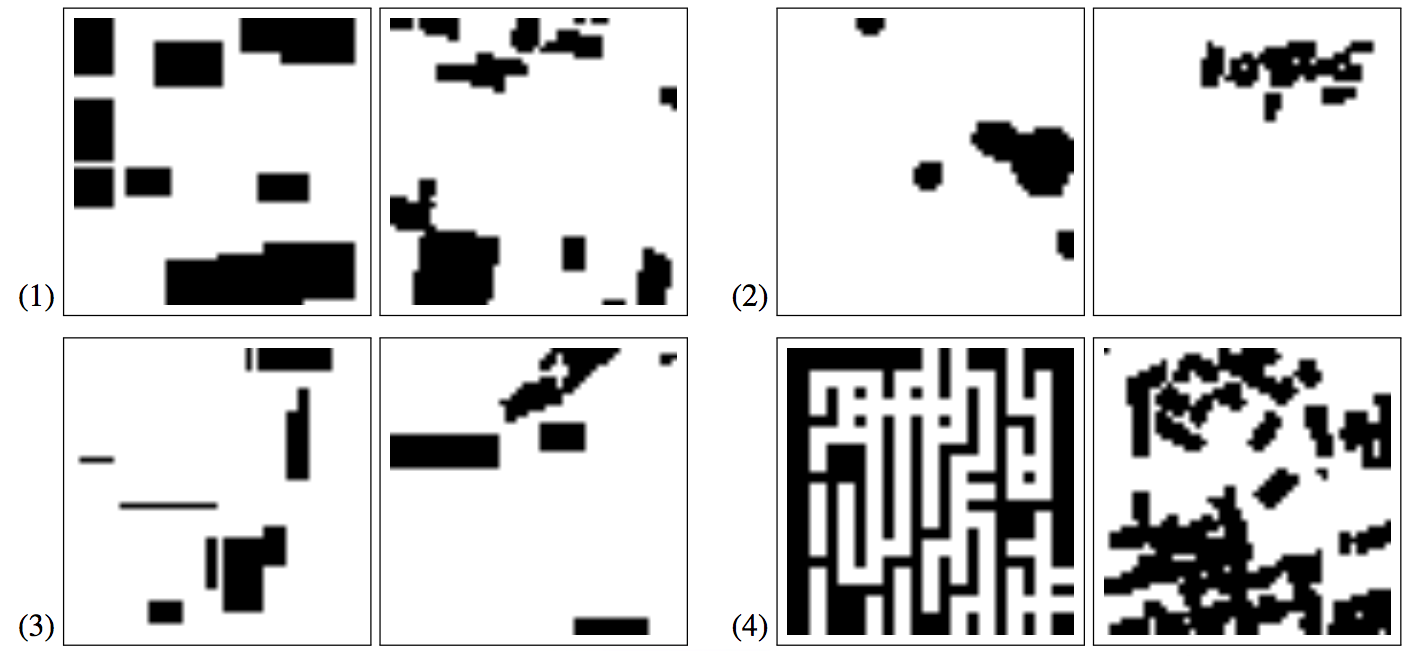
\includegraphics[width=0.63\textwidth]{figures/spatialsens_calib.png}
		\hspace{0.5cm}
		
\includegraphics[width=0.29\textwidth]{figures/mesobench_Fig3.png}
		
		\end{center}
		
		{\small\textit{Left: buildings \cite{raimbault2019generating}; Right: population \cite{raimbault2020comparison}}}
		
          \end{column}
          \end{columns}
        \end{block}
        
        
         \begin{block}{Urban evolution}
       \vspace{-2cm}
        \begin{columns}[t]
        \begin{column}{.95\textwidth}
        
        \vspace{0.5cm}
        
        \textit{Urban evolutionary theory introduced by \cite{pumain1997pour}}
        
        
  		\vspace{1cm}
        
        An \textbf{explicit urban evolution model} described by \cite{raimbault2020model}:
		\begin{itemize}
			\item Spatial diffusion of innovations captures transmission processes
			\item Spatial interaction models drive innovation and population growth
			\item Urban genome as the distribution of different innovations
			\item Mutation as the emergence of new innovations
		\end{itemize}

        \bigskip
        
        % trim=0cm 20cm 0cm 0cm trim does not work
        \begin{center}
        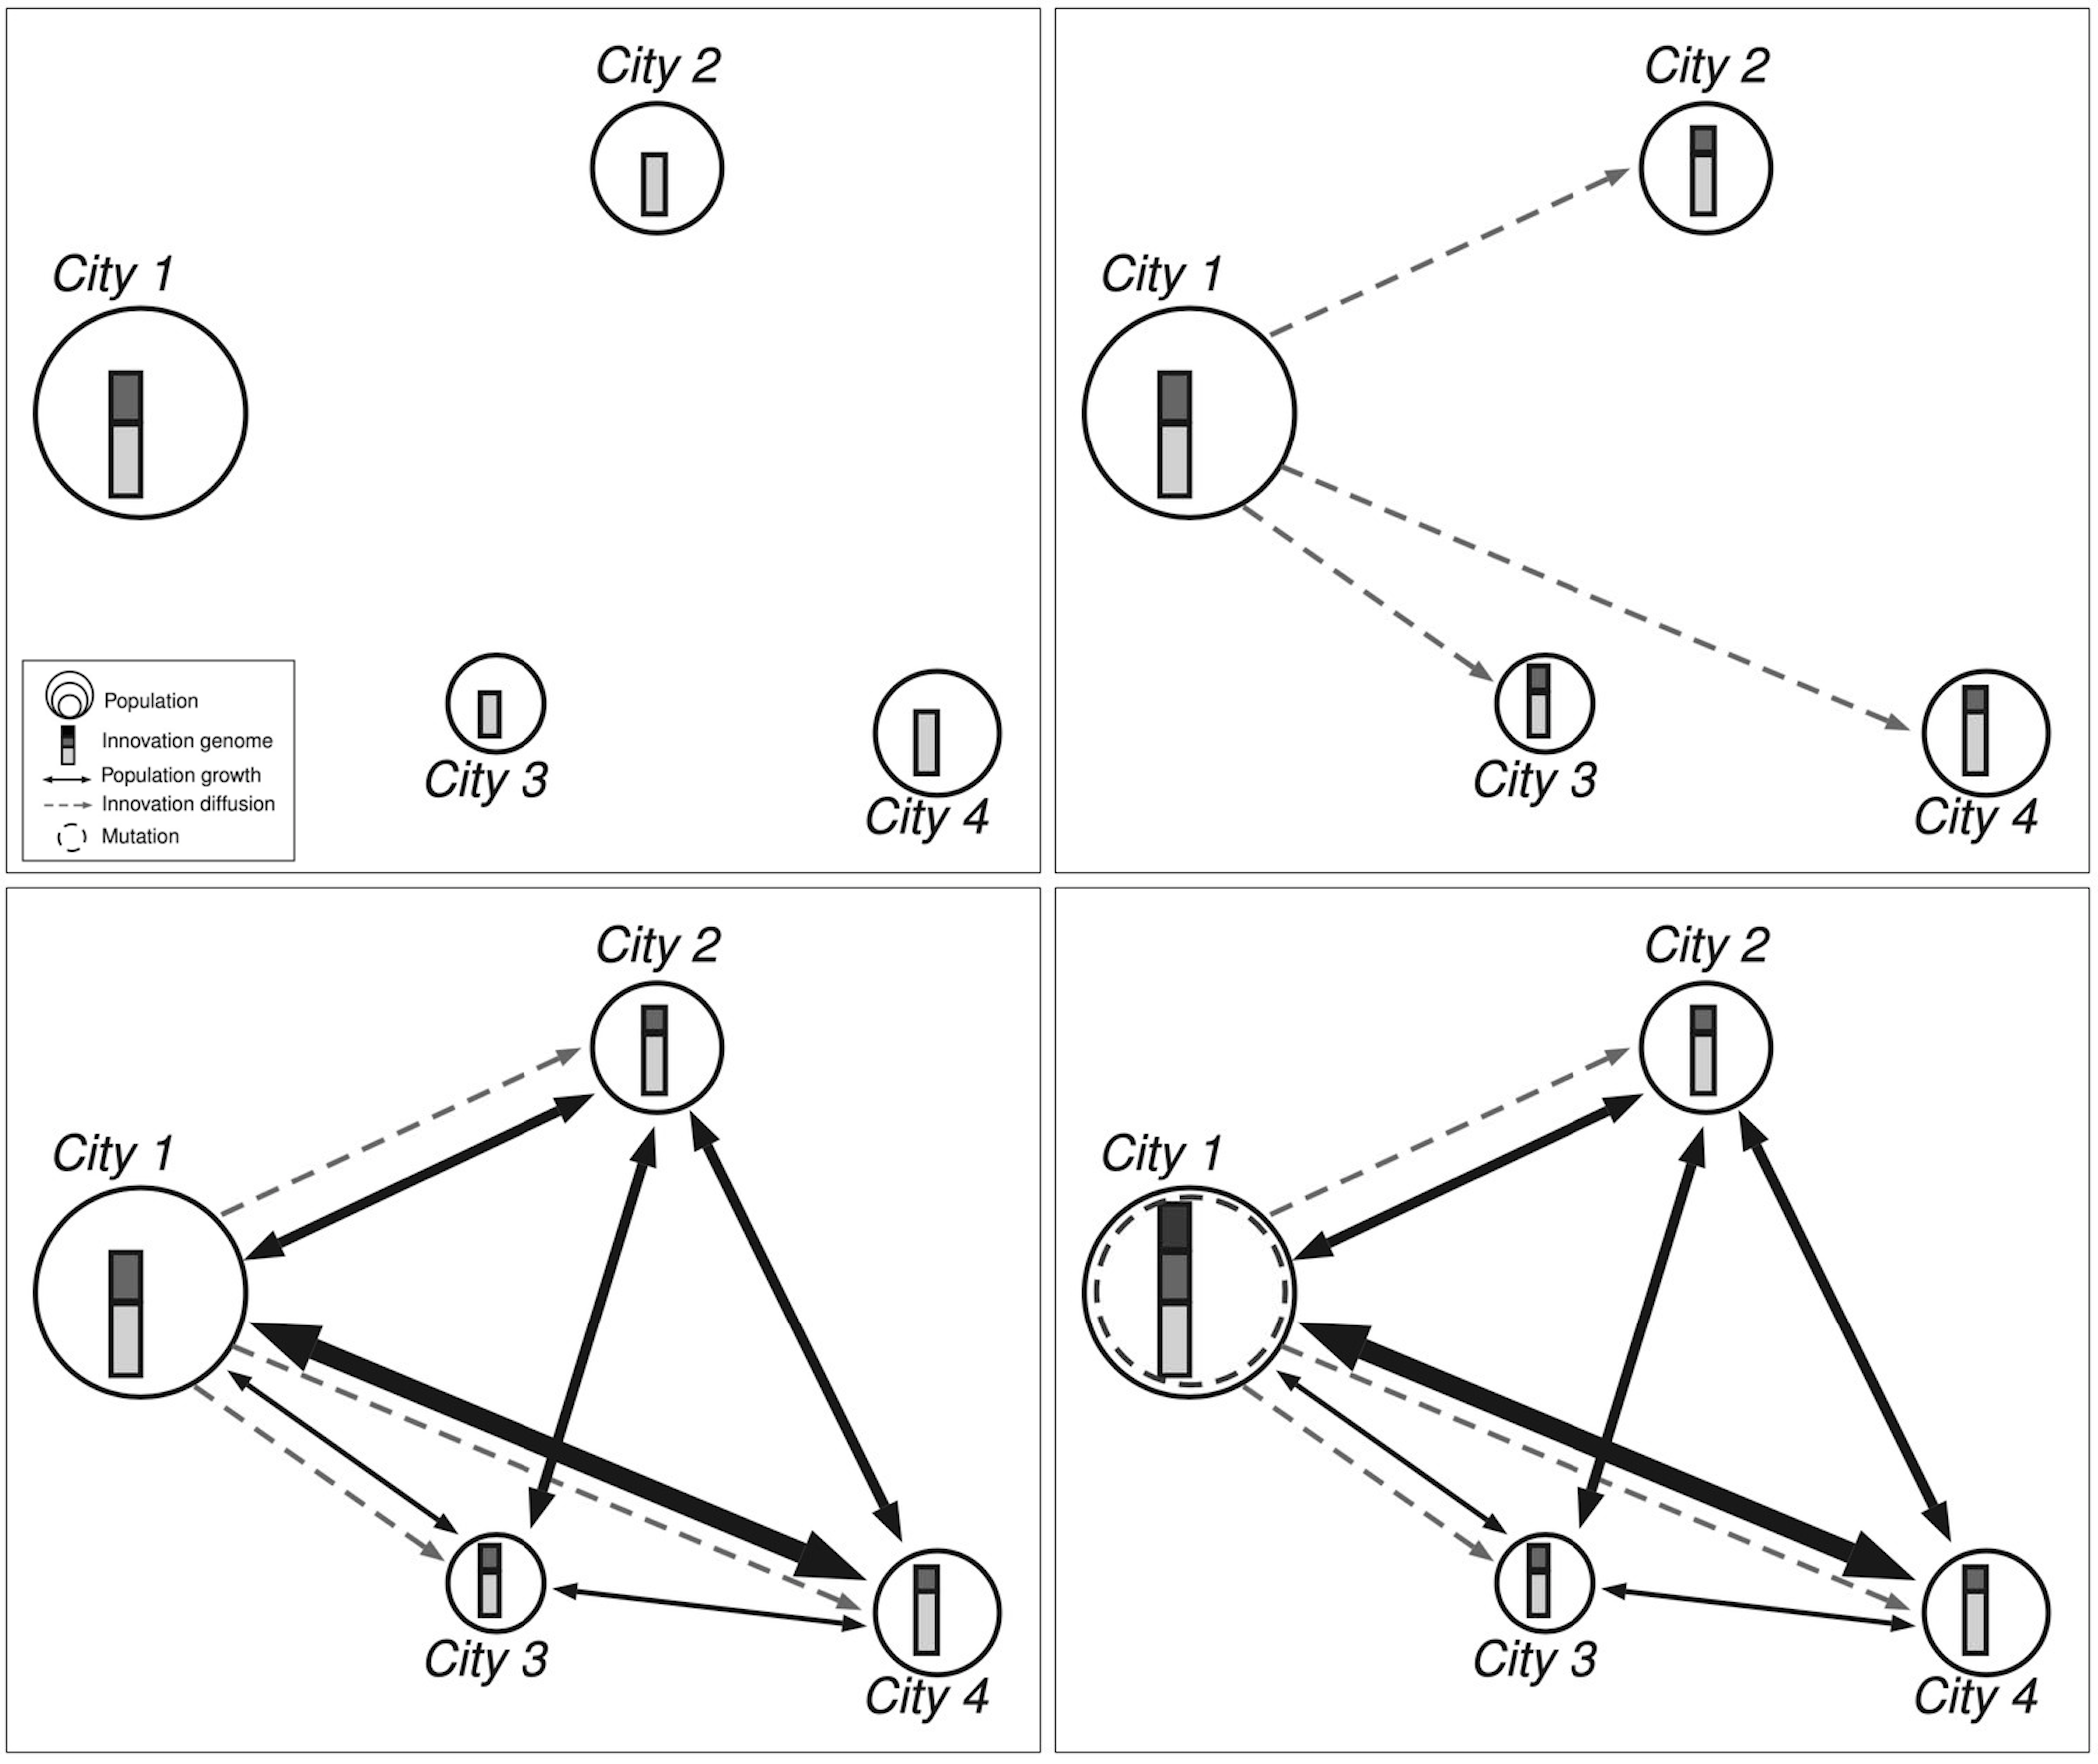
\includegraphics[width=\textwidth]{figures/urbanevol_Fig2.png}
        
        {\small\textit{Processes in the urban evolution model \cite{raimbault2020spatial}}}
        
        \end{center}
        
        
          \end{column}
          \end{columns}
        \end{block}

        
      
      \end{column}
      
      
      
      \begin{column}{.49\textwidth}
      
      \vspace{-1cm}
      
      
       
    
        
      
      
      
       \begin{block}{Co-evolution in urban systems}
        \vspace{-1.5cm}
          \begin{columns}[t]
        \begin{column}{.95\textwidth}
        
        
        
       %\begin{justify} 
       
       \textbf{Definition of urban co-evolution} \cite{raimbault2018caracterisation}: \textit{statistically co-evolving population of urban entities within territorial niches}
       
       \vspace{1cm}
       
       \textbf{Characterisation method} based on circular Granger causalities between proxy variables
       
       \bigskip
       
       \begin{center}
       \includegraphics[width=0.87\textwidth]{figures/carac_regimes_1.png}
       
       {\small \textit{Diverse causality regimes in a morphogenesis model \cite{raimbault2017identification}}}
       \end{center}
       
       
       \vspace{1cm}
       
       \textbf{Application} to transportation networks and territories:
       
       \bigskip
       
       \begin{itemize}
       		\item At the \textbf{mesoscopic} scale (urban areas), co-evolution of urban morphology and road network topology \cite{raimbault2019urban}
       \end{itemize}
       \begin{center}
       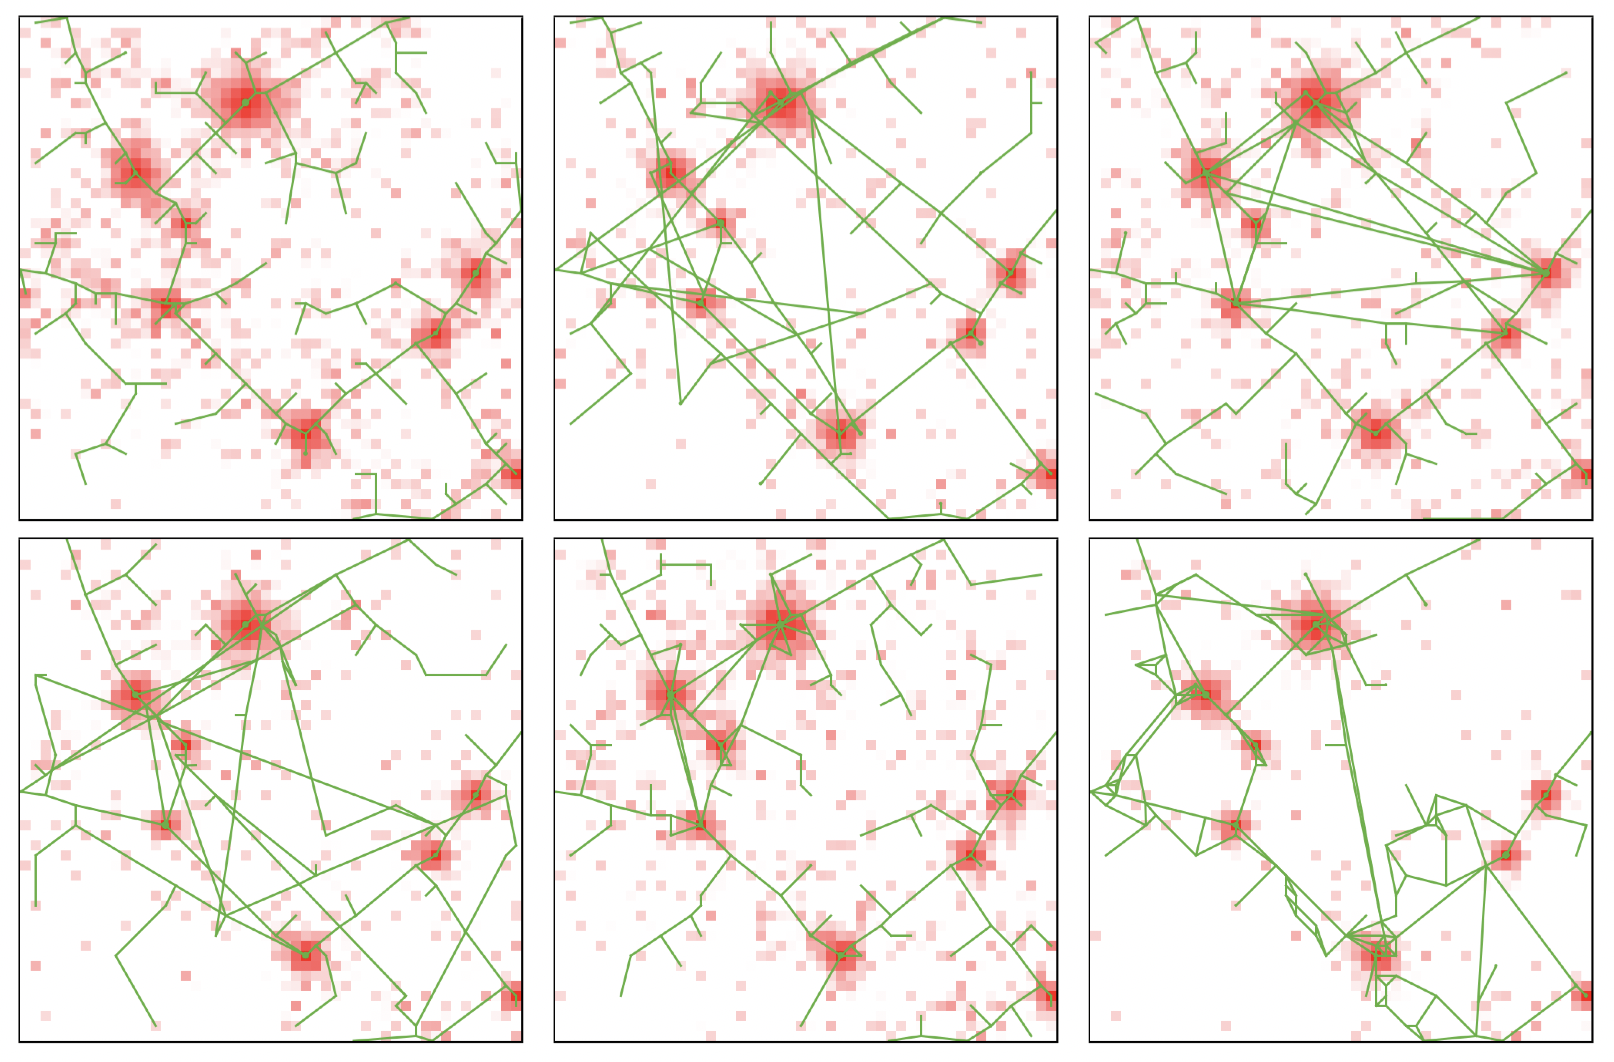
\includegraphics[width=0.87\textwidth]{figures/meso_multimodeling.png}
       
       {\small \textit{Multiple network growth heuristics \cite{raimbault2018multi}}}
       
		\end{center}

        \vspace{1cm}
        
        \begin{itemize}
        	\item Land-use transport model and transportation governance at the \textbf{urban region} scale \cite{raimbault2021introducing}	
        \end{itemize}
        
        \vspace{1cm}
        
        \begin{itemize}
        	\item At the \textbf{macroscopic} scale (systems of cities), co-evolution between cities and inter-city transport networks \cite{raimbault2021modeling}
        \end{itemize}

       
       \vspace{1cm}
       
       \textbf{Possible extensions:} application to other urban dimensions (mobility and accessibility e.g.), integration with explicit urban evolution models
      
       
       %\end{justify}
         
         
        
        
                  \end{column}
          \end{columns}
        \end{block}
      
      
      
        \begin{block}{Discussion}
         \begin{columns}[t]
        \begin{column}{.95\textwidth}

		\vspace{-1.5cm}

		\begin{itemize}
			\item \justify Potential transfer of other concepts to urban systems: biomimicry, autopoiesis, collective computation
		\end{itemize}
		
		\begin{itemize}
			\item \justify Towards multi-scale models for urban systems
		
		\end{itemize}
		
		\begin{itemize}
			\item \justify Application to sustainable policies at multiple spatial and time scales \cite{rozenblat2018conclusion}
		\end{itemize}
          
          \end{column}
          \end{columns}
        \end{block}
        
        
        
      \end{column}
    \end{columns}
    
    %\begin{columns}[t]
    %  \begin{column}{\linewidth}
    
    \begin{block}{References}
        {\tiny
        \vspace{-1cm}
        \begin{multicols}{4}
          \bibliographystyle{apalike}
          \bibliography{biblio}
        \end{multicols}
          }
        \end{block}
    %\end{column}
    %\end{columns}
    
  \end{frame}
\end{document}





